\documentclass[letterpaper,12pt]{article}
\usepackage[bottom=2.5cm, top=2.5cm, right=2cm, left=3cm]{geometry}
\usepackage[spanish, es-tabla]{babel}
\usepackage{graphicx} 
\usepackage{hyperref}
\usepackage{booktabs}
\usepackage{natbib}
\usepackage{float}
\usepackage{listings}
\usepackage{xcolor}
\usepackage{parskip} 
\usepackage{fancyhdr} % Paquete para personalizar encabezados y pies de página
\usepackage{microtype}  % Mejora la justificación del texto

\hypersetup{
    colorlinks=true,
    linkcolor=black,
    citecolor=black,
    urlcolor=blue
}

% Configuración del encabezado
\pagestyle{fancy}
\fancyhf{} % Limpia los encabezados y pies de página actuales
\fancyhead[R]{\thepage} % Coloca el número de página en la parte superior derecha
\renewcommand{\headrulewidth}{0pt} % Elimina la línea horizontal en la parte superior de la página

\begin{document}

\begin{titlepage}
    \begin{center}
        
    
    \vspace*{1cm}


    \textbf{\Large EVALUACIÓN SOCIAL BASADA EN REALIDAD}
  
    \vspace{1cm}
    
    \textbf{Bernardo Caprile Canala-Echevarría, Felipe Alberto Vicencio Fossa y Lukas Wolff Casanova}\\
    Facultad de Ingeniería y Ciencias Aplicadas, Universidad de los Andes, Santiago de Chile\\
    e-mail: \href{mailto:bcaprile@miuandes.cl}{bcaprile@miuandes.cl}, \href{mailto:favicencio@miuandes.cl}{favicencio@miuandes.cl}, \href{mailto:lwolff@miuandes.cl}{lwolff@miuandes.cl}\\
    GitHub: \href{https://github.com/LukasWolff2002/TAREA_4_AUTITOS}{Repositorio}
    \vspace{2cm}
    
    \textbf{RESUMEN}
    \end{center}
    \vspace{0.5cm}
    
    %Acá va el resumen


    \vspace{1cm}
    
    \textit{Palabras clave:} \textit{}
    
\end{titlepage}

\newpage
\section{Introducción}

En este informe se tiene como objetivo evaluar socialmente la mejora de una propuesta en una red vial ficticia, inspirada en el sector de San Carlos de Apoquindo. El grafo de la Figura \ref{fig:imagen1} representa dicha red, donde los diferentes arcos y centroides simbolizan avenidas y puntos clave de la zona. 


\begin{figure}[h]
    \centering
    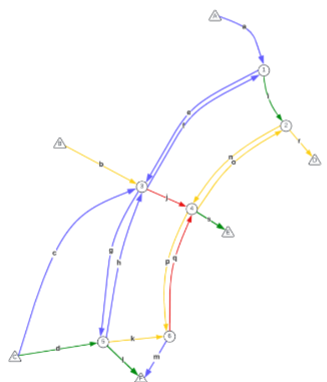
\includegraphics[width=0.3\textwidth]{FOTOS/diagrama.png}
    \caption{Diagrama de la red vial ficticia}
    \label{fig:imagen1}
\end{figure}



La mejora propuesta consiste en reorganizar las avenidas General Blanche y Camino El Alba para operar en sentidos exclusivos (oriente y poniente, respectivamente), permitiendo la delimitación de tres pistas en cada vía y reduciendo conflictos de tránsito. Este cambio implica una modificación en la función de costo del arco $d$, que pasa a formar parte del conjunto amarillo con un parámetro $S = 2000$.

El análisis considera las metodologías de evaluación social vistas en clase, con un enfoque en los beneficios derivados de la reducción de tiempos de viaje durante horas punta. En los apartados siguientes, se detallan los datos base, la metodología aplicada, los cálculos realizados y las conclusiones obtenidas.

\newpage
\section{Resultados}
\subsection{Datos de la propuesta base}


\begin{table}[h!]
    \centering
    \begin{tabular}{ccccccc}
        \toprule
        \textbf{Arco} & \textbf{Flujo [veh]} & \textbf{Costo aprox. [h]} & \textbf{CTi} & \textbf{CC} & \textbf{OC} \\
        \midrule
        a & 1600.00 & 0.625 & 2.017872e+09 & 2.559557e+08 & 1.523648e+08 \\
        b & 2250.00 & 0.150 & 6.810318e+08 & 1.176139e+08 & 2.142630e+08 \\
        c & 1255.00 & 0.280 & 7.090802e+08 & 1.025944e+08 & 1.195111e+08 \\
        d & 1845.00 & 0.255 & 9.493583e+08 & 1.403678e+08 & 1.756956e+08 \\
        e & 710.31  & 0.025 & 3.583287e+07 & 1.699836e+07 & 6.764139e+07 \\
        f & 610.03  & 0.025 & 3.077406e+07 & 1.459857e+07 & 5.809193e+07 \\
        g & 605.30  & 0.025 & 3.053545e+07 & 1.448537e+07 & 5.764150e+07 \\
        h & 0.02    & 0.025 & 1.008936e+03 & 4.786180e+02 & 1.904560e+03 \\
        i & 1499.72 & 0.025 & 7.565607e+07 & 3.588965e+07 & 1.428153e+08 \\
        j & 3000.00 & 0.025 & 1.513404e+08 & 7.179270e+07 & 2.856840e+08 \\
        k & 785.28  & 0.025 & 3.961486e+07 & 1.879246e+07 & 7.478063e+07 \\
        l & 1665.00 & 0.135 & 4.535672e+08 & 8.137159e+07 & 1.585546e+08 \\
        m & 1085.00 & 0.110 & 2.408330e+08 & 4.687573e+07 & 1.033224e+08 \\
        n & 89.69   & 0.025 & 4.524573e+06 & 2.146362e+06 & 8.540998e+06 \\
        o & 1089.97 & 0.025 & 5.498550e+07 & 2.608396e+07 & 1.037956e+08 \\
        p & 694.70  & 0.025 & 3.504539e+07 & 1.662480e+07 & 6.615488e+07 \\
        q & 394.98  & 0.025 & 1.992548e+07 & 9.452227e+06 & 3.761315e+07 \\
        r & 2500.00 & 0.275 & 1.387287e+09 & 2.015371e+08 & 2.380700e+08 \\
        s & 1700.00 & 0.158 & 5.420004e+08 & 9.194747e+07 & 1.618876e+08 \\
        \bottomrule
    \end{tabular}
    \caption{Tabla de datos de flujo, costo aproximado y costos adicionales de la propuesta incial}
    \label{tab:datos_actualizados}
\end{table}

\newpage
\subsection{Datos de la propuesta mejorada}
\begin{table}[h!]
    \centering
    \begin{tabular}{ccccccc}
        \toprule
        \textbf{Arco} & \textbf{Flujo [veh]} & \textbf{Costo aprox. [h]} & \textbf{CTi} & \textbf{CC} & \textbf{OC} \\
        \midrule
        a & 1600.00 & 0.625 & 2.017872e+09 & 2.559557e+08 & 1.523648e+08 \\
        b & 2250.00 & 0.150 & 6.810318e+08 & 1.176139e+08 & 2.142630e+08 \\
        c & 1050.00 & 0.075 & 1.589074e+08 & 3.703107e+07 & 9.998938e+07 \\
        d & 2050.00 & 0.050 & 2.068319e+08 & 6.067855e+07 & 1.952174e+08 \\
        e & 710.31  & 0.025 & 3.583287e+07 & 1.699836e+07 & 6.764139e+07 \\
        f & 610.03  & 0.025 & 3.077406e+07 & 1.459857e+07 & 5.809193e+07 \\
        g & 605.30  & 0.025 & 3.053545e+07 & 1.448537e+07 & 5.764150e+07 \\
        h & 102.52  & 0.025 & 5.171806e+06 & 2.453396e+06 & 9.762773e+06 \\
        i & 1499.72 & 0.025 & 7.565607e+07 & 3.588965e+07 & 1.428153e+08 \\
        j & 2897.50 & 0.025 & 1.461696e+08 & 6.933978e+07 & 2.759231e+08 \\
        k & 887.78  & 0.025 & 4.478566e+07 & 2.124537e+07 & 8.454150e+07 \\
        l & 1665.00 & 0.135 & 4.535672e+08 & 8.137159e+07 & 1.585546e+08 \\
        m & 1085.00 & 0.110 & 2.408330e+08 & 4.687573e+07 & 1.033224e+08 \\
        n & 89.69   & 0.025 & 4.524573e+06 & 2.146362e+06 & 8.540998e+06 \\
        o & 1089.97 & 0.025 & 5.498550e+07 & 2.608396e+07 & 1.037956e+08 \\
        p & 694.70  & 0.025 & 3.504539e+07 & 1.662480e+07 & 6.615488e+07 \\
        q & 497.48  & 0.025 & 2.509627e+07 & 1.190514e+07 & 4.737402e+07 \\
        r & 2500.00 & 0.275 & 1.387287e+09 & 2.015371e+08 & 2.380700e+08 \\
        s & 1700.00 & 0.158 & 5.420004e+08 & 9.194747e+07 & 1.618876e+08 \\
        \bottomrule
    \end{tabular}
    \caption{Tabla de datos de flujo, costo aproximado y costos adicionales de la propuesta mejorada}
    \label{tab:datos}
\end{table}

\begin{table}[h!]
    \centering
    \begin{tabular}{ccccc}
        \toprule
        \textbf{Arco} & \textbf{Variación CTi} & \textbf{Variación CC} & \textbf{Variación OC} \\
        \midrule
        a & 0.0         & 0.000000e+00 & 0.000000e+00 \\
        b & 0.0         & 0.000000e+00 & 0.000000e+00 \\
        c & 550172800.8 & 6.556331e+07 & 1.952174e+07 \\
        d & 742526449.2 & 7.968926e+07 & -1.952174e+07 \\
        e & 0.0         & 0.000000e+00 & 0.000000e+00 \\
        f & 0.0         & 0.000000e+00 & 0.000000e+00 \\
        g & 0.0         & 0.000000e+00 & 0.000000e+00 \\
        h & -5170797.0  & -2.452917e+06 & -9.760868e+06 \\
        i & 0.0         & 0.000000e+00 & 0.000000e+00 \\
        j & 5170797.0   & 2.452917e+06 & 9.760868e+06 \\
        k & -5170797.0  & -2.452917e+06 & -9.760868e+06 \\
        l & 0.0         & 0.000000e+00 & 0.000000e+00 \\
        m & 0.0         & 0.000000e+00 & 0.000000e+00 \\
        n & 0.0         & 0.000000e+00 & 0.000000e+00 \\
        o & 0.0         & 0.000000e+00 & 0.000000e+00 \\
        p & 0.0         & 0.000000e+00 & 0.000000e+00 \\
        q & -5170797.0  & -2.452917e+06 & -9.760868e+06 \\
        r & 0.0         & 0.000000e+00 & 0.000000e+00 \\
        s & 0.0         & 0.000000e+00 & 0.000000e+00 \\
        \bottomrule
    \end{tabular}
    \caption{Variación de los costos por arco.}
    \label{tab:variacion_costos}
\end{table}


\begin{table}[h!]
    \centering
    \begin{tabular}{ccc}
        \toprule
        \textbf{Costo del Proyecto} & \textbf{Variación Total de Costos} & \textbf{Ganancia Obtenida} \\
        \midrule
        1,000,000,000 & 1,403,182,654.38 & 403,182,654.38 \\
        \bottomrule
    \end{tabular}
    \caption{Resumen tabular de costos y ganancias del proyecto.}
    \label{tab:resumen_costos}
\end{table}


\end{document}